\section{Data and methodology}\label{sec:methodology}

This section presents the proposed data sources and methodology of the thesis. \S\ref{subsec:data-sources} introduces the Universal Dependencies treebanks as well as additional resources that will be used as reference and validation in this study. The rest of the section, \S\ref{subsec:features}-\ref{subsec:infotheory}, presents the main computational methods to be used in the thesis.

\subsection{Data sources}\label{subsec:data-sources}

\textbf{Universal Dependencies (UD)} is designed to be a cross-linguistically consistent system for annotating morphosyntactic information within a dependency grammar framework \citep{demarneffe2021}. The UD treebanks \citep{universaldep} is the collection of cross-lingual treebanks annotated in the UD framework by an open community of more than 300 contributors. See \ref{tab:treebanks} for a table of languages available in UD v2.5, as an example.

\begin{table}[t]{}
    \centering
\begin{adjustbox}{center,scale=0.85}
\footnotesize
\renewcommand{\tabcolsep}{3pt}
    \begin{tabular}{|lrrr|lrrr|lrrr|}
    \hline
    \textbf{Language}  & \textbf{\#} & \textbf{Sents} & \textbf{Words} & \textbf{Language}  & \textbf{\#} & \textbf{Sents} & \textbf{Words} & \textbf{Language}  & \textbf{\#} & \textbf{Sents} & \textbf{Words} \\
    \hline
Afrikaans &1 &1,934 &49,276 &German &4 &208,440 &3,753,947 &Old Russian &2 &17,548 &168,522 \\
Akkadian &1 &101 &1,852 &Gothic &1 &5,401 &55,336 &Persian &1 &5,997 &152,920 \\
Amharic &1 &1,074 &10,010 &Greek &1 &2,521 &63,441 &Polish &3 &40,398 &499,392 \\
Ancient Greek &2 &30,999 &416,988 &Hebrew &1 &6,216 &161,417 &Portuguese &3 &22,443 &570,543 \\
Arabic &3 &28,402 &1,042,024 &Hindi &2 &17,647 &375,533 &Romanian &3 &25,858 &551,932 \\
Armenian &1 &2502 &52630 &Hindi English &1 &1,898 &26,909 &Russian &4 &71,183 &1,262,206 \\
Assyrian &1 &57 &453 &Hungarian &1 &1,800 &42,032 &Sanskrit &1 &230 &1,843 \\
Bambara &1 &1,026 &13,823 &Indonesian &2 &6,593 &141,823 &Scottish Gaelic &1 &2,193 &42,848 \\
Basque &1 &8,993 &121,443 &Irish &1 &1,763 &40,572 &Serbian &1 &4,384 &97,673 \\
Belarusian &1 &637 &13,325 &Italian &6 &35,481 &811,522 &Skolt S\'ami &1 &36 &321 \\
Bhojpuri &1 &254 &4,881 &Japanese &4 &67,117 &1,498,560 &Slovak &1 &10,604 &106,043 \\
Breton &1 &888 &10,054 &Karelian &1 &228 &3,094 &Slovenian &2 &11,188 &170,158 \\
Bulgarian &1 &11,138 &156,149 &Kazakh &1 &1,078 &10,536 &Spanish &3 &34,693 &1,004,443 \\
Buryat &1 &927 &10,185 &Komi Permyak &1 &49 &399 &Swedish &3 &12,269 &206,855 \\
Cantonese &1 &1,004 &13,918 &Komi Zyrian &2 &327 &3,463 &Swedish Sign Language &1 &203 &1,610 \\
Catalan &1 &16,678 &531,971 &Korean &3 &34,702 &446,996 &Swiss German &1 &100 &1,444 \\
Chinese &5 &12,449 &285,127 &Kurmanji &1 &754 &1,0260 &Tagalog &1 &55 &292 \\
Classical Chinese &1 &15,115 &74,770 &Latin &3 &41,695 &582,336 &Tamil &1 &600 &9,581 \\
Coptic &1 &1,575 &40,034 &Latvian &1 &13,643 &219,955 &Telugu &1 &1,328 &6,465 \\
Croatian &1 &9,010 &199,409 &Lithuanian &2 &3,905 &75,403 &Thai &1 &1,000 &22,322 \\
Czech &5 &127,507 &2,222,163 &Livvi &1 &125 &1,632 &Turkish &3 &9,437 &91,626 \\
Danish &1 &5,512 &100,733 &Maltese &1 &2,074 &44,162 &Ukrainian &1 &7,060 &122,091 \\
Dutch &2 &20,916 &306,503 &Marathi &1 &466 &3,849 &Upper Sorbian &1 &646 &11,196 \\
English &7 &35,791 &620,509 &Mby\'a Guaran\'i &2 &1,144 &13,089 &Urdu &1 &5,130 &138,077 \\
Erzya &1 &1,550 &15,790 &Moksha &1 &65 &561 &Uyghur &1 &3,456 &40,236 \\
Estonian &2 &32,634 &465,015 &Naija &1 &948 &12,863 &Vietnamese &1 &3,000 &43,754 \\
Faroese &1 &1,208 &10,002 &North S\'ami &1 &3,122 &26,845 &Warlpiri &1 &55 &314 \\
Finnish &3 &34,859 &377,619 &Norwegian &3 &42,869 &666,984 &Welsh &1 &956 &16,989 \\
French &7 &45,074 &1,157,171 &Old Church Slavonic &1 &6,338 &57,563 &Wolof &1 &2,107 &44,258 \\
Galician &2 &4,993 &164,385 &Old French &1 &17,678 &170,741 &Yoruba &1 &100 &2,664 \\
\hline
    \end{tabular}
\end{adjustbox}
    \caption{Languages in UD v2.5 with number of treebanks (\#), sentences (Sents) and words (Words).}
    \label{tab:treebanks}
\end{table}

A subset of the UD treebanks, the \textbf{Parallel Universal Dependencies (PUD)} treebanks were originally developed for the CoNLL-2017 Shared Task \citep{zeman2017} and include 1000 sentences in 18 languages that were randomly picked from newswire and Wikipedia and annotated according to UD v2 guidelines. The 18 languages are English, German, French, Italian, Spanish, Arabic, Hindi, Chinese, Indonesian, Japanese, Korean, Portuguese, Russian, Thai, Turkish, Czech, Finnish and Swedish. Of the sentences, 750 were originally English, while the remaining 250 sentences come from German, French, Italian and Spanish texts and translated to other languages through English. While facing obvious limitation in terms of language coverage, corpus size, and possible artifacts due to the so-called ``translationese'', parallel corpora allow for cross-lingual comparison with a smaller data size and will also be considered in this thesis.

In additional to the main data source of UD treebanks, additional resources will be used in the study as reference and to perform validation and evaluation of the intermediate results. As an example, the valency frames and verb classes as induced from the UD treebanks will be validated, where possible, against the expert-annotated data from \textbf{the Valency Patterns Leipzig Online Database (ValPaL)} \citep{valpal}. Other datasets will be introduced as necessary.

\subsection{Representing verb instances / feature selection}\label{subsec:features}

In the first step, the specific uses of verbs are abstracted through a feature selection process. Each instance of verb use will be represented by the morphosyntactic features of the sentence, namely only features that are considered part of valency frame encoding are included. This is in order to focus on whether semantically coherent verb classes can be induced from valency frame information alone. In selecting the features, cross-lingual differences in valency frame coding will be taken into account, e.g., whether a language uses morphological cases or word order to encode valency frame information. Word order information, although not explicitly specified in UD, should also be extracted from the dataset. An alternative approach considered is to keep manual feature selection at a minimum and to allow the clustering algorithms to weigh the features as needed.

\subsection{Clustering}\label{subsec:clustering}

The clustering process after feature selection consists of two steps, but the clustering algorithms used need not be the same. The first is the automatic induction of valency frames in a language given the selected features and the second is the clustering of verbs, represented by their distribution over the valency frames, into verb classes. Since unsupervised clustering will be used, the number of valency frames and the number of verb classes cannot be assumed \textit{a priori}. This requires either using algorithms that do not require a predefined number of clusters (e.g., Ward clustering), or experimenting with cluster sizes with each language (cf. \cite{schulteimwalde2006}, which used the k-means algorithm with a predefined the gold standard number). Due to the lack the gold standard for many of the languages to be experimented on, the former seems preferable. A bottom-up agglomerative clustering method will also be favored over top-down methods.

Given the relative low dimensionality of hand-selected features, complex clustering algorithms are not anticipated to be necessary. Nevertheless, more modern clustering algorithms should also be investigated \citep{xu2015a}. Given the two levels of clustering, one method to be considered for the verb class induction is the Hierarchical Dirichlet process, which is particularly suited for clustering grouped data (cf. \citet{parisien2010}, Fig.~\ref{fig:parisien2010}, where a Hierarchical Dirichlet process was extended to account for diathesis alternations).

\begin{figure}
    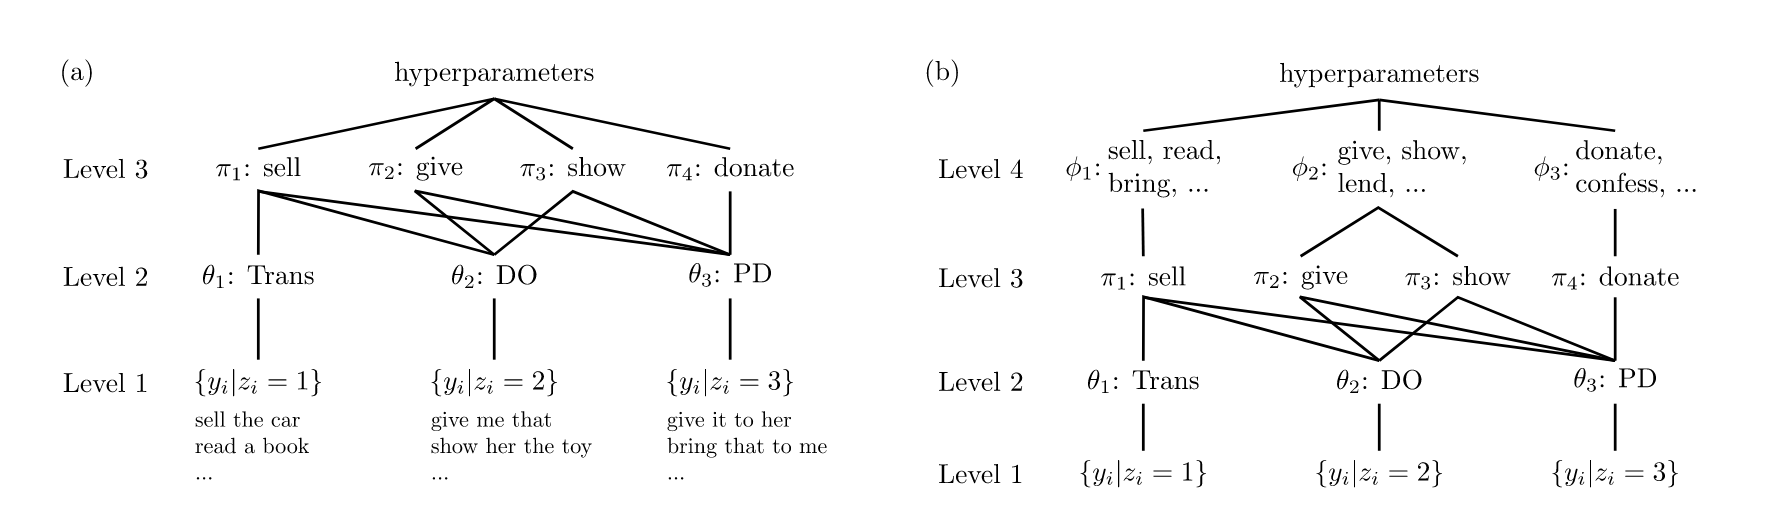
\includegraphics[width=\textwidth]{figures/verb_alternation_classes.png}
    \centering
    \caption{(a) Model 1, a Hierarchical Dirichlet Process applied to learning verb argument structure constructions. (b) Model 2,
    an extension of Model 1 to learn verb alternation classes.}\label{fig:parisien2010}
\end{figure}

\subsection{Cross-lingual verb sense alignment}\label{subsec:verblist}

A cross-lingual aligned list of counterpart verbs will be needed to compare the verb classes. The easiest way to do this is likely through existing cross-lingual word lists such as LanguageNet, part of the PanLex project \citep{kamholz2014}. However, multilingual word embeddings and induction of a cross-lingual verbal lexicon could be considered as another option should the existing resources prove insufficient.

\subsection{Information theory metrics}\label{subsec:infotheory}

The specific metrics to be used on the results will have to be determined in combination with the decisions to be made in the experiments such as the number of the language studied and whether parallel or non-parallel datasets are used. Preliminarily, however, information theory metrics modeled on those used by \citet{say2014} are considered, specifically an internal complexity metric measuring the entropy of the distribution of verbs among valency classes and a similarity metric based on mutual information measuring the similarity / dissimilarity between valency systems of two or more languages.